\section{Interpolación cuadrática}

En la práctica se pide implementar la interpolación cuadrática para hacer que los saltos de una plataforma a otra sigan una parábola. A diferencia de la interpolación lineal, esta requiere usar un punto adicional, que es un punto intermedio.

\bigskip

Hay varias formas de realizar la interpolación cuadrática: la más famosa es la interpolación de Lagrange, que para grado 2 es fácil de calcular. Otra opción es utilizar la fórmula de las curvas Bézier para obtener la parábola.

\bigskip

He optado por utilizar la segunda opción porque parecía más fácil de implementar, ya que teníamos la interpolación lineal ya programada. Por tanto, los puntos pasan a ser puntos de control, que al ser unidos se obtienen dos segmentos. A dichos segmentos hay que aplicarles la interpolación lineal con el mismo factor, obteniéndose así dos puntos que forman otro segmento, al que a su vez hay que aplicarle interpolación lineal con el mismo factor que antes. Realizando esto todas las veces que sea necesario, se obtiene una parábola.

\bigskip

Cabe destacar que el objeto no pasará por el punto intermedio, ya que es un punto de control por el que no puede pasar, pero si pasará por el punto de inicio y el final.

% imagen de la animacion esa de wikipedia
\begin{figure}[H]
   \centering
   \includegraphics[width=0.7\textwidth]{imagenes/Bézier_2_big.png}
   \caption{Visualización de la interpolación realizada con un factor de interpolación de 0,7\cite{enwiki:1153684109}.}
\end{figure}

\begin{figure}[H]
    \centering
    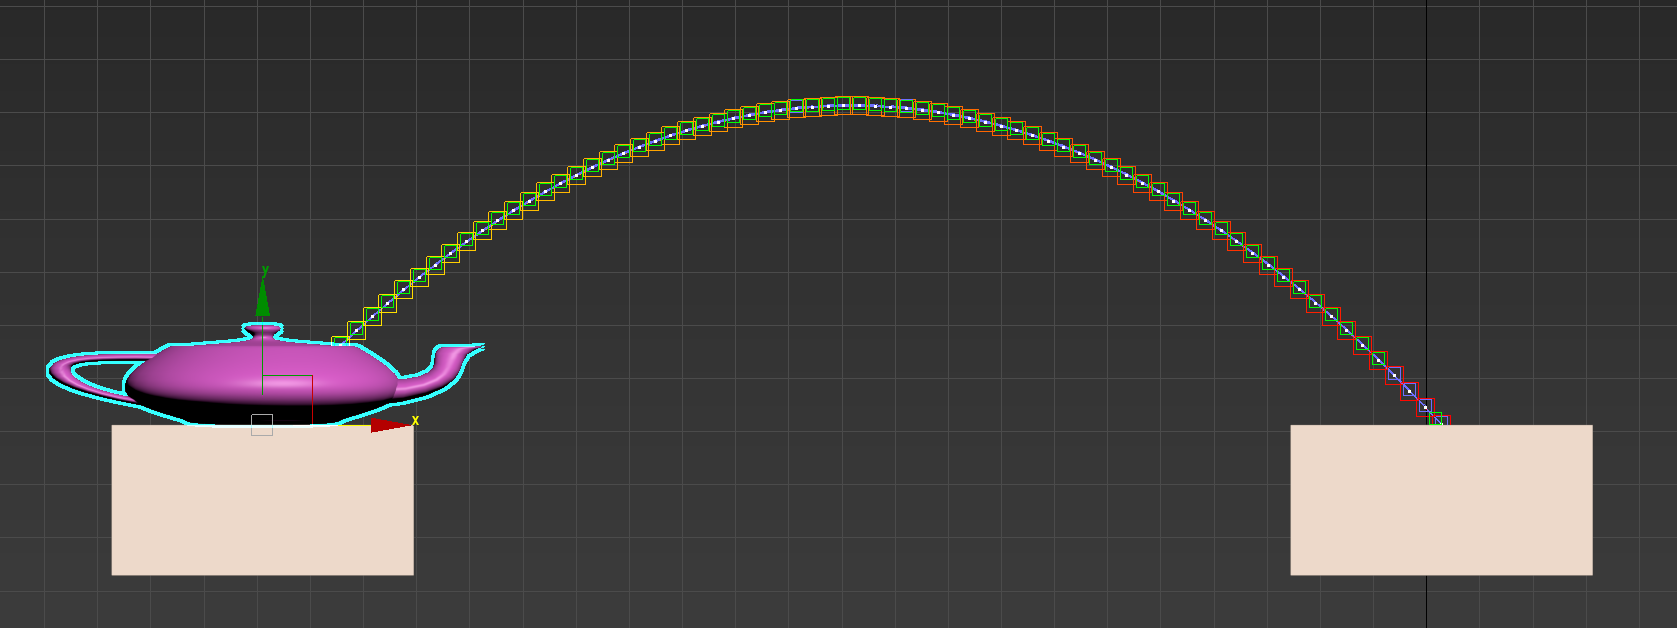
\includegraphics[width=0.8\textwidth]{imagenes/motion path.png}
    \caption{Trayectoria resultante entre dos plataformas con la misma altura.}
 \end{figure}